% !TEX encoding = UTF-8
% !TEX TS-program = pdflatex
% !TEX root = ../tesi.tex

\chapter{Fast Broadcast}
	\label{chapter:fb}
	Fast Broadcast \cite{4199282} is a multi-hop routing protocol for vehicular communication. Its main feature consists in breaking the assumption that all vehicles should know, a priori, their fixed and constant transmission range. This assumption is often unreasonable, especially in \acrshort{vaneta}s and urban environments, where electromagnetic interferences and obstacles such as buildings heavily influence the transmission range.
	
	
	Fast Broadcast employs two different phases:
	\begin{enumerate}
		\item the \textbf{Estimation Phase}, during which cars estimate their frontward and backward transmission range;
		\item the \textbf{Broadcasts Phase}, during which a car sends an Alert Message and the other cars need to forward it in order to propagate the information.
	\end{enumerate}

	\section{Estimation Phase}
		During this phase, cars try to estimate their frontward and backward transmission range by the means of Hello Messages. These beacons are sent periodically via broadcast to all the neighbors of a vehicle.
		
		
		Time is divided into turns and, in order to keep estimations fresh, data collected during a certain turn is kept for the duration of the next turn, then discarded. The parameter \textit{turnSize} specifies the duration of a turn: the authors suggest a duration of one second. A bigger \textit{turnSize} could guarantee less collisions to the detriment of freshness of information. On the other hand, the effects of a smaller \textit{turnSize} are specular to those just presented. 
		
		
		Using this approach, vehicles can estimate two different values:
		\begin{itemize}
			\item \textit{Current-turn Maximum Front Range (CMFR)}, which estimates the maximum frontward distance from which another car can be heard by the considered one;
			\item \textit{Current-turn Maximum Back Range} (CMBR), which estimates the maximum backward distance at which the considered car can be heard.
		\end{itemize}
		When the turn expires, the value of these variables is stored in the LMFR and LMBR variables (\textit{Latest-turn Maximum Front Range} and \textit{Latest-turn Maximum Back Range}, respectively). The algorithm uses both last turn and current turn data because the former guarantees values calculated with a larger pool of Hello Messages, while the latter considers fresher information.
		
		When sending a Hello Message (Algorithm \ref{alg:hello-message-sending}), the vehicle initially waits for a random time between 0 and \textit{turnSize}. After this, if it has not heard another Hello Message or a collision, it proceeds to transmit a Hello Message containing the estimation of its frontward transmission range.
		
		
		When receiving a Hello Message (Algorithm \ref{alg:hello-message-receiving}), the vehicle retrieves its position and the sender's position, calculates the distance between these two positions and then updates the CMFR field if the message comes from ahead, otherwise CMBR is updated. The new value is obtained as the maximum between the old CMFR or CMBR value, the distance between the vehicle and the sender, and the sender's transmission range estimation included in the Hello Message.
		
		\begin{algorithm}[H]
			\begin{algorithmic}[1]
				\ForEach{turn}
					\State sendingTime $\gets$ random(turnSize)
					\State wait(sendingTime)
					\If{$\neg$ (heardHelloMsg() $\lor$ heardCollision())}
						\State helloMsg.declaredMaxRange $\gets$ max(LMFR, CMFR)
						\State transmit(helloMsg)
					\EndIf
				\EndFor
			\end{algorithmic}
			\caption{Hello message sending procedure}
			\label{alg:hello-message-sending}
		\end{algorithm}
		
		\begin{algorithm}[H]
			\begin{algorithmic}[1]
				\State mp $\gets$ myPosition()
				\State sp $\gets$ helloMsg.senderPosition
				\State drm $\gets$ helloMsg.declaredMaxRange
				\State d $\gets$ distance(mp, sp)
				\If{receivedFromFront(helloMsg)} 
				\State CMFR $\gets$ max(CMFR, d, drm)
				\Else
				\State CMBR $\gets$ max(CMBR, d, drm)
				\EndIf
			\end{algorithmic}
			\caption{Hello message receiving procedure}
			\label{alg:hello-message-receiving}
		\end{algorithm}
	
	\section{Broadcast Phase}
		This phase is activated once a car sends an Alert Message. The other cars can exploit the estimation of transmission ranges to reduce redundancy in message broadcast. Each vehicle can exploit this information to assign itself a forwarding priority inversely proportional to the relative distance: the higher the relative distance, the higher the priority.  
		
		
		When the Broadcast Phase is activated , a vehicle sends an Alert Message with application specific data. Broadcast specific data is also piggybacked on the Alert Message, such as:
		\begin{itemize}
			\item \textit{MaxRange:} the maximum range a transmission is expected to travel backward before the signal becomes too weak to be received. This value is utilized by following vehicles to rank their forwarding priority;
			\item \textit{SenderPosition}: the coordinates of the sender.
		\end{itemize}
		Upon reception, each vehicle waits for a random time called \textit{Contention Window} (\textit{CW}). This window ranges from a minimum value (\textit{CWMin}) and a maximum one (\textit{CWMax}) depending on sending/forwarding car distance (\textit{Distance}) and on the estimated transmission range (\textit{MaxRange}), according to formula \ref{eq:contention-window}. It is quite easy to see that the higher the sender/forwarder distance is, the lower the contention window is.
		\begin{gather}
			\left\lfloor \left( \frac{\text{MaxRange} - \text{Distance}}{\text{MaxRange}} \times (\text{CWMax} - \text{CWMin}) \right) + \text{CWmin}  \right\rfloor
			\label{eq:contention-window}
		\end{gather}
		If another forwarding of the same message coming from behind is heard during waiting time, the vehicle suppresses its transmission because the message has already been forwarded by another vehicle further back in the column. On the contrary, if the same message is heard coming from the front, the procedure is restarted using the new parameters. The vehicle can forward the message only if the waiting time expires without having received the same message.
		
		Algorithm \ref{alg:alert-message-generation} and \ref{alg:alert-message-forwarding} describe the logic behind the Broadcast Phase.
		
		\begin{algorithm}[H]
			\begin{algorithmic}[1]
				\State alertMessage.maxRange $\gets$ max(LMBR, CMBR)
				\State alertMessage.position $\gets$ retrievePosition()
				\State transmit(alertMessage) $\gets$ helloMsg.declaredMaxRange
			\end{algorithmic}
			\caption{Alert Message generation procedure}
			\label{alg:alert-message-generation}
		\end{algorithm}
	
		\begin{algorithm}[H]
			\begin{algorithmic}[1]
				\State cwnd $\gets$ computeCwnd()
				\State waitTime $\gets$ retrievePosition()
				\State wait(waitTime
				\If{sameBroadcastHeardFromBack()}
				\State exit()
				\ElsIf{sameBroadcastHeardFromFront()}
				\State restartBroadcastProcedure()
				\Else 
				\State maxRange $\gets$ max(LMBR, CMBR)
				\EndIf 
			\end{algorithmic}
			\caption{Alert Message generation procedure}
			\label{alg:alert-message-forwarding}
		\end{algorithm}
	
	\section{Two dimensions extension}
		The original work \cite{4199282} considered only a strip-shaped road, where it was easy to define directions and establish 	when a message came from the front or the back. In \cite{BAR2017} an extension considering two dimensions was proposed. 
		
		
		The modifications to the Fast Broadcast algorithm are the following:
		\begin{enumerate}
			\item Utilizing only one parameter between CMBR and CMFR (thus considering only CMR):
			\item Including the position of the vehicle which originally generated the Alert Message in addition to the position of the sender of the message.
		\end{enumerate}
		
		
		When a vehicle receives an Alert Message, the origin-vehicle distance is confronted with the origin-sender distance: the vehicle can forward the message only if the former is greater than or equal to the latter, otherwise it simply discards the message.
		
		\begin{figure}[H]
			\centering
			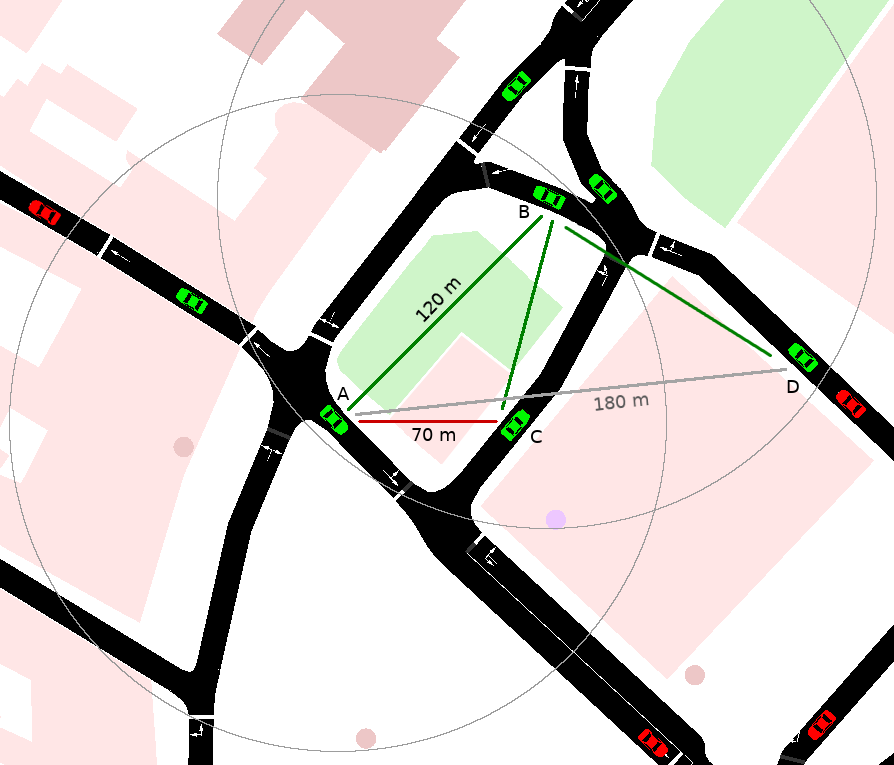
\includegraphics[width=\textwidth]{immagini/fb-2dpicc}
			\caption{Example of Fast Broadcast in 2d scenario}
			\label{fig:fb-2d}
		\end{figure}
		
		
		
		For example, suppose that vehicle A is the origin of the Alert Message and B receives it, but C doesn't due to an obstacle in the line of sight. B computes origin-vehicle distance, $d(A, B)$, and origin-sender distance, $d(A, A)$, which in this case are respectively 120 and 0m. Since origin-vehicle is greater than origin-sender, B can forward the Alert Message.
		
		
		Now suppose that C receives the message from B. C computes origin-vehicle distance, $d(A, C)$, and origin-sender distance, $d(A, B)$, which amount to 70 and 120m respectively. Since the former is not greater than or equal to the latter, C is not a candidate for forwarding and suppresses the transmission.
		
		
		D receives the message from B as well. D is a good candidate for transmission since the origin-vehicle distance, which amounts to 180m, is greater than origin-sender distance, equal to 120m.
%todo inserire struttura pacchetto
% todo rimuovere riferimenti alle distanze